% This is LLNCS.DEM the demonstration file of
% the LaTeX macro package from Springer-Verlag
% for Lecture Notes in Computer Science,
% version 2.4 for LaTeX2e as of 16. April 2010
%
\documentclass[10pt,a4paper]{article}
%\documentclass{llncs}
%
%\synctex=1

\usepackage[linesnumbered,ruled,vlined]{algorithm2e}

%\usepackage[T1]{fontenc}
%\usepackage{lmodern}

\usepackage{graphicx}
\usepackage{epsfig}

\usepackage{array}
%\setlength{\extrarowheight}{0pt}


%\usepackage{bigstrut}
%    \setlength\bigstrutjot{3pt}


\usepackage{amssymb}
%\usepackage{MnSymbol}
\usepackage{bm}
\usepackage{amsmath}

\usepackage{bussproofs}
\usepackage[USenglish]{babel}

\usepackage{subfigure}

\usepackage{times}

\usepackage{booktabs}

\usepackage{float}

\usepackage{multirow}


\usepackage{todonotes}

%\usepackage[T1]{fontenc}
%\usepackage{cmbright}


% \fontencoding{T1}
%  \fontfamily{garamond}
%  \fontseries{m}
%  \fontshape{it}
%  \fontsize{12}{15}
%  \selectfont

% correct bad hyphenation here
\hyphenation{op-tical net-works semi-conduc-tor}

\newcommand{\code}[1]{{\fontfamily{cmtt}\small\selectfont#1}}
\newcommand{\codefs}[1]{{\fontfamily{cmtt}\scriptsize\selectfont#1}}


%\usepackage{fancyvrb}
%\DefineVerbatimEnvironment{codenv}{Verbatim}{fontfamily=ssf}
%cmss
%{\begin{Verbatim}[fontfamily=cmss]}%
%{\end{Verbatim}}%

% multiline comments
\usepackage{verbatim}

\usepackage{color}
\usepackage{listings}

%  basicstyle=\sffamily\small,


\lstdefinelanguage{Scala}{
	morekeywords={},
	morekeywords=[2]{
		public, private, protected,
		abstract,case,catch,class,def,
		do,else,extends,false,final,finally,
		for,if,implicit,import,match,mixin,
		new,null,object,override,package,
		private,protected,requires,return,sealed,
		super,this,throw,trait,true,try,
		type,val,var,while,with,yield,
		lazy,evt,observable,imperative,
                after,before},
	otherkeywords={=>,<-,<\%,<:,>:,\#,@},
	sensitive=true,
	morecomment=[l]{//},
	morecomment=[n]{/*}{*/},
	morestring=[b]",
	morestring=[b]',
	morestring=[b]"""
}
\lstloadlanguages{Scala}

\lstset{
  backgroundcolor=\color{white},%\fontfamily{cmtt}
  basicstyle=\fontfamily{cmtt}\footnotesize,
  basewidth=0.5em,
  showstringspaces=false,
  keywordstyle=\fontfamily{pcr}\color[rgb]{0,0,0}\bfseries,
  %commentstyle=\color[rgb]{0.133,0.545,0.133},
  %stringstyle=\color[rgb]{0.627,0.126,0.941},
  breaklines=false,
  frame=none
  breaklines=false,
  frame=none,
  numbers=left, numberstyle=\tiny, stepnumber=1, numbersep=5pt,
  %frameround=fttt,
  %frame=single,
  escapeinside={(*@}{@*)},
  %columns=fullflexible
}


\lstnewenvironment{codenv}{\lstset{language=Scala}}{}
\lstnewenvironment{codenvOpt}[1]{\lstset{language=Scala,#1}}{}


\newenvironment{bluetext}{\color{blue}}{\ignorespacesafterend}
\newenvironment{redtext}{\color{red}}{\ignorespacesafterend}
\newcommand{\bygerold}[1]{ \begin{bluetext} #1 \end{bluetext}}
\newcommand{\commentbygerold}[1]{\\\begin{redtext} #1 \end{redtext}\\}

%\newenvironment{codenv}{\small \begin{itshape}}{ \end{itshape}}



%\renewcommand*{\bibfont}{\footnotesize}



% Avoid (not that) big pictures alone in a blank page
\renewcommand{\topfraction}{0.85}
\renewcommand{\textfraction}{0.1}
\renewcommand{\floatpagefraction}{0.75}

\usepackage{xspace}
\newcommand{\REScala}{{\small \sc{REScala}}\xspace}


\newcommand{\mm}[1]{\todo[color=green!40]{#1}}
\newcommand{\jd}[1]{\todo[color=blue!40]{#1}}
\newcommand{\gs}[1]{\todo[color=red!40]{#1}}

\usepackage{color}


\hyphenation{Res-ca-la}


\newcommand{\str}[1]{{\sf\selectfont @#1@}\newline}





\title{REScala Reference Manual}


\author{Guido Salvaneschi\\ Technical University of Darmstadt\\
\code{salvaneschi@informatik.tu-darmstadt.de}\\}


\date{November 2013\\ \vspace*{10mm} Version 0.2}



\begin{document}

\maketitle
\newpage
\pagenumbering{Roman}
\tableofcontents
%\newpage
%\listoffigures
%\newpage
%\listoftables
\newpage
\pagenumbering{arabic}





\section{Introduction}

This manual covers the main features of the \REScala programming
language. Section~\ref{sec:sig-and-vars} presents time-changing values
in \REScala, Section~\ref{sec:events} describes events,
Section~\ref{sec:conv-fun} covers the conversion functions between
events and time-changing values, Section~\ref{sec:technicalities}
presents technical details that are necessary to correctly run
\REScala, Section~\ref{sec:related} outlines the related work.


\paragraph{Intended audience and prerequisites} This manuscript is
mainly intended for students who approach reactive programming in
Scala for the first time.  The manual assumes basic knowledge of the
Scala~\cite{scala} language and of functional programming (high-order
functions, anonymous functions, etc.). No previous knowledge of
reactive programming is assumed.

While a major aspect of \REScala's design is the integration of events
and signals, they can be used separately. For example a programmer can
use only \REScala events to design application that do not need
time-changing values.

\paragraph{Scope} The manual covers the basic features of
\REScala. Some functionalities, including implicit events and
high-order signals are intentionally not covered, other, like event
polymorphism, are only sketched. More details can be found
in~\cite{rescala,Gasiunas:2011:EME:1960275.1960303}.

The manual introduces the concepts related to functional reactive
programming and event-based programming from a practical
perspective. The readers interested in a more general presentation of
these topics can find in Section~\ref{sec:related} the essential
references.



\newpage






\section{Signals and Vars}\label{sec:sig-and-vars}

A signal is language concept for expressing functional dependencies
among values in a declarative way. Intuitively, a reactive value can
depend on variables -- sources of change without further dependencies
-- or on other reactive values.  When any of the dependency sources
changes, the expression defining the reactive value is automatically
recomputed by the language runtime to keep the reactive value
up-to-date.

Consider the following example:

\begin{codenv}
var a = 2
var b = 3
var c = a + b   (*@\label{sum}@*)
println(a,b,c) // -> (2,3,5)
a = 4
println(a,b,c) // -> (2,4,5) (*@\label{nomore}@*)
c = a + b (*@\label{update}@*)
println(a,b,c) // -> (4,3,7)
\end{codenv}

Line~\ref{sum} specifies the value of \code{c} as a function of
\code{a} and \code{b}. Since Line~\ref{sum} defines a {\it statement},
the relation $c = a + b$ is valid after the execution of
Line~\ref{sum}. Clearly, when the value of \code{a} is updated, the
relation $c = a + b$ is not valid anymore (Line~\ref{nomore}). To make
sure that the relation still holds, the programmer needs to recompute
the expression and reassign \code{c}, like in line \ref{update}.
\\

Reactive programming and \REScala provide abstractions to express {\em
  constraints} in addition to statements. In \REScala, the programmer
can specify that the constraint $c := a + b$ {\em always} holds during
the execution of a program. Every time \code{a} or \code{b} change,
the value of \code{c} is automatically recomputed.

For example:
\begin{codenv}
val a = Var(2)
val b = Var(3)
val c = Signal{ a() + b() }   (*@\label{sumS}@*)
println(a.get,b.get,c.get) // -> (2,3,5)
a()= 4  (*@\label{updated}@*)
println(a.get,b.get,c.get) // -> (4,3,7)
\end{codenv}

In the code above, the signal in Line~\ref{sumS} defines the
constraint $c := a + b$. When one of the reactive values involved in
the constraint is updated (Line~\ref{updated}), the expression in the
constraint is recomputed behind the scenes, and the value of \code{a}
is automatically updated.

As the reader may have noticed, expressing constraints in \REScala
requires to conform some syntactic conventions which are discussed in
the next sections.


\subsection{Vars}


\subsubsection{Defining Vars} Programmers express reactive
computations starting from vars. Vars wrap normal Scala values. For
example, \code{Var(2)} creates a var with an \code[Int] value and
initializes the var to the value 2. Vars are parametric types. A var
that carries integer values has type \code{Var[Int]}. The following
code snippet shows valid var declarations.

\begin{codenv}
val a = Var(0)
val b = Var("Hello World")
val c = Var(false)
val d: Var[Int] = Var(30)
val e: Var[String] = Var("REScala")
val f: Var[Boolean] = Var(false)
\end{codenv}


\subsubsection{Assigning Vars} Vars can be directly modified with the
\code{()=} operator. For example \code{v()=3} replaces the current
value of the \code{v} var with \code{3}. Therefore, vars are changed
imperatively by the programmer.



\subsection{Signals}

\subsubsection{Defining Signals} Signals are defined by the syntax
\code{Signal\{}{\it sigexpr}\code{\}}, where {\it sigexpr} is a side
effect-free expression. Signals are parametric types. A signal that
carries integer values has the type \code{Signal[Int]}.

\subsubsection{Signal expressions} When, inside a signal expression
defining a signal \code{s}, a var or a signal is called with the
\code{()} operator, the var or the signal are added to the values
\code{s} depends on. In that case, \code{s} {\it is a dependency} of
the vars and the signals in the signal expression. For example in the
code snippet:

\begin{codenv}
  val a = Var(0)
  val b = Var(0)
  val s = Signal{ a() + b() } // Multiple vars in a signal expression
\end{codenv}

The signal \code{s} is a dependency of the vars \code{a} and \code{b},
meaning that the values of \code{s} depends on both \code{a} and
\code{b}. The following code snippets define valid signal
declarations.

\begin{codenv}
val a = Var(0)
val b = Var(0)
val c = Var(0)
val r: Signal[Int] = Signal{ a() + 1 } // Explicit type in var decl
val s = Signal{ a() + b() } // Multiple vars is a signal expression
val t = Signal{ s() * c() + 10 } // Mix signals and vars in signal expressions
val u = Signal{ s() * t() } // A signal that depends on other signals
\end{codenv}

\begin{codenv}
val a = Var(0)
val b = Var(2)
val c = Var(true)
val s = Signal{ if (c()) a() else b() }
\end{codenv}

\begin{codenv}
def factorial(n: Int) = ...
val a = Var(0)
val s: Signal[Int] = Signal{ // A signal expression can be any code block
  val tmp = a() * 2
  val k = factorial(tmp)
  k + 2  // Returns an Int
}
\end{codenv}



\subsubsection{Accessing reactive values} The current value of a
signal or a var can be accessed using the \code{get} method. For
example:

\begin{codenv}
val a = Var(0)
val b = Var(2)
val c = Var(true)
val s: Signal[Int] = Signal{ a() + b() }
val t: Signal[Boolean] = Signal{ !c() }
val x: Int = a.get
val y: Int = s.get
val z: Boolean = t.get
println(z)
\end{codenv}



\subsection{Example: speed}
The following example computes the displacement \code{space} of a
particle that is moving at constant speed \code{SPEED}. The
application prints all the values associated to the displacement over
time.

\begin{codenv}
val SPEED = 10
val time = Var(0)
val space = Signal{ SPEED * time() } (*@\label{sigexpr}@*)

space.changed += ((x: Int) => println(x)) (*@\label{conversion}@*)

while (true) {
  Thread sleep 20
  time() = time.get + 1  (*@\label{increasetime}@*)
}

-- output --
10
20
30
40
 ...
\end{codenv}


The application behaves as follows. Every 20 milliseconds, the value
of the \code{time} var is increased by 1 (Line~\ref{increasetime}).
When the value of the \code{time} var changes, the signal expression
at Line~\ref{sigexpr} is reevaluated and the value of \code{space} is
updated. Finally, the current value of the \code{space} signal is
printed every time the value of the signal changes.

Printing the value of a signal deserves some more considerations.
Technically, this is achieved by converting the \code{space} signal to
an event that is fired every time the signal changes its value
(Line~\ref{conversion}). The conversion is performed by the
\code{changed} operator. The \code{+=} operator attaches an handler to
the event returned by the \code{changed} operator. When the event
fires, the handler is executed. Line~\ref{conversion} is equivalent to
the following code:

\begin{codenv}
val e: Event[Int] = space.changed
val handler:  (Int => Unit) =  ((x: Int) => println(x))
e += handler
\end{codenv}


Note that using \code{println(space.get)} would also print the
value of the signal, but only at the point in time in which the print
statement is executed. Instead, the approach described so far prints
{\it all} values of the signal. More details about converting signals
into events and back are provided in Section~\ref{sec:conv-fun}.


\newpage





\section{Events}\label{sec:events}

\REScala supports different kind of events. Imperative events are
directly triggered from the user. Declarative events trigger when the
events they depend on trigger. In reactive applications, events are
typically used to model changes that happen at discrete points in
time. For example a mouse click from the user or the arrival of a new
network packet. Some features of \REScala events are valid for all
event types.

\begin{itemize}

\item Events carry a value. The value is associated to the event when
  the event is fired and received by all the registered handlers when
  each handler is executed.

\item Events are generic types parametrized with the type of value
  they carry, like \code{Event[T]} and \code{ImpertiveEvent[T]} where
  \code{T} is the value carried by the event.

\item Both imperative events and declarative events are subtypes of
  \code{Event[T]} and can referred to generically.

\end{itemize}

\subsection{Imperative events}

\REScala imperative events are triggered imperatively by the
programmer. One can think to imperative events as a generalization of
a method call which supports (multiple) bodies that are registered and
unregistered dynamically.

\subsubsection{Defining  Events}

Imperative events are defined by the \code{ImperativeEvent[T]}
type. The value of the parameter \code{T} defines the value that is
attached to the event. An event with no parameter attached has
signature \code{ImpertiveEvent[Unit]}. The following code snippet show
valid events definitions:

\begin{codenv}
val e1 = new ImperativeEvent[Unit]()
val e2 = new ImperativeEvent[Int]()
val e3 = new ImperativeEvent[String]()
val e4 = new ImperativeEvent[Boolean]()
val e5: ImperativeEvent[Int] = new ImperativeEvent[Int]()
class Foo
val e6 = new ImperativeEvent[Foo]()
\end{codenv}

It is possible to attach more than one value to the same event. This
is easily accomplished by using a tuple as a generic parameter
type. For example:

\begin{codenv}
val e1 = new ImperativeEvent[(Int,Int)]()
val e2 = new ImperativeEvent[(String,String)]()
val e3 = new ImperativeEvent[(String,Int)]()
val e4 = new ImperativeEvent[(Boolean,String,Int)]()
val e5: ImperativeEvent[(Int,Int)] = new ImperativeEvent[(Int,Int)]()
\end{codenv}

Note that an imperative event is also an event. Therefore the
following declaration is also valid:

\begin{codenv}
val e1: Event[Int] = new ImperativeEvent[Int]()
\end{codenv}



\subsubsection{Registering Handlers}

Handlers are code blocks that are executed when the event fires. The
\code{+=} operator attaches the handler to the event. The handler is a
first class function that receives the attached value as a parameter.
The following are valid handler definitions.

\begin{codenv}
var state = 0
val e = new ImperativeEvent[Int]()
e += { println(_) }
e += (x => println(x))
e += ((x: Int) => println(x))
e += (x => {  // Multiple statements in the handler
  state = x
  println(x)
})
\end{codenv}

The signature of the handler must conform the signature of the event,
since the handler is supposed to process the attached value and
perform side effects. For example is the event is of type
\code{Event[(Int,Int)]} the handler must be of type \code{(Int,Int) =>
  Unit}.

\begin{codenv}
val e = new ImperativeEvent[(Int,String)]()
e += (x => {
  println(x._1)
  println(x._2)
})
e += (x: (Int,String) => {
  println(x)
})
\end{codenv}

Note that events without arguments still need a \code{Unit} argument
in the handler.

\begin{codenv}
val e = new ImperativeEvent[Int]()
e += { x => println() }
e += { (x: Unit) => println() }
\end{codenv}

Scala allows one to refer to a method using the partially applied
function syntax. This approach can be used to directly register a
method as an event handler. For example:

\begin{codenv}
def m1(x: Int) = {
  val y = x + 1
  println(y)
}
val e = new ImperativeEvent[Int]
e += m1 _
e(10)
\end{codenv}



\subsubsection{Firing Events}

Events can be fired with the same syntax of a method call. When an
event is fired, a proper value must be associated to the event
call. Clearly, the value must conform the signature of the event. For
example:

\begin{codenv}
val e1 = new ImperativeEvent[Int]()
val e2 = new ImperativeEvent[Boolean]()
val e3 = new ImperativeEvent[(Int,String)]()
e1(10)
e2(false)
e3((10,"Hallo"))
\end{codenv}

When a handler is registered to an event, the handler is executed
every time the event is fired. The actual parameter is provided to the
handler.

\begin{codenv}
val e = new ImperativeEvent[Int]()
e += { x => println(x) }
e(10)
e(10)
-- output ----
10
10
\end{codenv}

If multiple handlers are registered, all of them are executed when the
event is fired. Applications should not rely on any specific execution
order for handler execution.

\begin{codenv}
val e = new ImperativeEvent[Int]()
e += { x => println(x) }
e += { x => println(f"n: $x")}  (*@\label{$}@*)
e(10)
e(10)
-- output ----
10
n: 10
10
n: 10
\end{codenv}






\subsubsection{Unregistering Handlers}

Handlers can be unregistered from events with the \code{-=}
operator. When a handler is unregistered, it is not executed when the
event is fired.

\begin{codenv}
val e = new ImperativeEvent[Int]()
val handler1 = { x: Int => println(x) }
val handler2 = { x: Int => println(s"n: $x") } (*@\label{$}@*)

e += handler1
e += handler2
e(10)
e -= handler2
e(10)
e -= handler1
e(10)

-- output ----
10
n: 10
10
\end{codenv}




\subsection{Declarative Events}

\REScala supports declarative events, which are defined as a
combination of other events. For this purpose it offers operators like
$e_1||e_2$ , $e_1\&\&p$ , $e_1.map(f)$. Event composition allows to
express the application logic in a clear and declarative way. Also,
the update logic is better localized because a single expression
models all the sources and the transformations that define an event
occurrence.


\subsubsection{Defining Declarative Events}

Declarative events are defined by composing other events. The
following code snippet shows some examples of valid definitions for
declarative events.

\begin{codenv}
val e1 = new ImperativeEvent[Int]()
val e2 = new ImperativeEvent[Int]()

val e3 = e1 || e2
val e4 = e1 && ((x: Int)=> x>10)
val e5 = e1 map ((x: Int)=> x.toString)
\end{codenv}


\subsection{Event Operators}

This section presents in details the operators that allow one to
compose events into declarative events.

\subsubsection{OR Events}

The event $e_1 || e_2$ is fired upon the occurrence of one among $e_1$
or $e_2$. Note that the events that appear in the event expression
must have the same parameter type (\code{Int} in the next example).

\begin{codenv}
val e1 = new ImperativeEvent[Int]()
val e2 = new ImperativeEvent[Int]()
val e1_OR_e2 = e1 || e2
e1_OR_e2 += ((x: Int) => println(x))
e1(10)
e2(10)
-- output ----
10
10
\end{codenv}


\subsubsection{Predicate Events}

The event $e \&\& p$ is fired if $e$ occurs and the predicate $p$ is
satisfied. The predicate is a function that accepts the event
parameter as a formal parameter and returns \code{Boolean}. In other
words the $\&\&$ operator filters the events according to their
parameter and a predicate.

\begin{codenv}
val e = new ImperativeEvent[Int]()
val e_AND: Event[Int] = e && ((x: Int) => x>10)
e_AND += ((x: Int) => println(x))
e(5)
e(15)
-- output ----
15
\end{codenv}


\subsubsection{Map Events}

The event $e\,map f$ is obtained by applying $f$ to the value carried
by $e$. The map function must take the event parameter as a formal
parameter. The return type of the map function is the type parameter
value of the resulting event.

\begin{codenv}
val e = new ImperativeEvent[Int]()
val e_MAP: Event[String] = e map ((x: Int) => x.toString)
e_MAP += ((x: String) => println(s"Here: $x")) (*@\label{$}@*)
e(5)
e(15)
-- output ----
Here: 5
Here: 15
\end{codenv}




\subsubsection{dropParam}

The $dropParam$ operator transforms an event into an event with
\code{Unit} parameter. In the following example the $dropParam$
operator transforms an \code{Event[Int]} into an \code{Event[Unit]}.

\begin{codenv}
val e = new ImperativeEvent[Int]()
val e_drop: Event[Unit] = e.dropParam
e_drop += (_ => println("*"))
e(10)
e(10)
-- output ----
*
*
\end{codenv}

The typical use case for the $dropParam$ operator is to make events
with different types compatible. For example the following snippet is
rejected by the compiler since it attempts to combine two events of
different types with the $||$ operator.

\begin{codenv}     /* WRONG - DON'T DO THIS */
val e1 = new ImperativeEvent[Int]()
val e2 = new ImperativeEvent[Unit]()
val e1_OR_e2 = e1 || e2  // Compiler error
\end{codenv}

The following example is correct. The $dropParam$ operator allows
one to make the events compatible with each other.

\begin{codenv}
val e1 = new ImperativeEvent[Int]()
val e2 = new ImperativeEvent[Unit]()
val e1_OR_e2: Event[Unit] = e1.dropParam || e2
\end{codenv}



\newpage



\section{Conversion Functions}\label{sec:conv-fun}

\REScala provides functions that interface signals and
events. Conversion functions are fundamental to introduce
time-changing values into OO applications -- which are usually
event-based.



\subsection{Basic Conversion Functions}

This section covers the basic conversions between signals and events.
Figure~\ref{fig:event-signal} shows how basic conversion functions can
bridge signals and events. Events (Figure~\ref{fig:event-signal},
left) occur at discrete point in time (x axis) and have an associate
value (y axis). Signals, instead, hold a value for a continuous
interval of time (Figure~\ref{fig:event-signal}, right). The
\code{latest} conversion functions creates a signal from an event. The
signal holds the value associated to an event. The value is hold until
the event is fired again and a new value is available. The
\code{changed} conversion function creates an event from a signal. The
function fires a new event every time a signal changes its value.



\begin{figure}[tp]
\begin{center}
  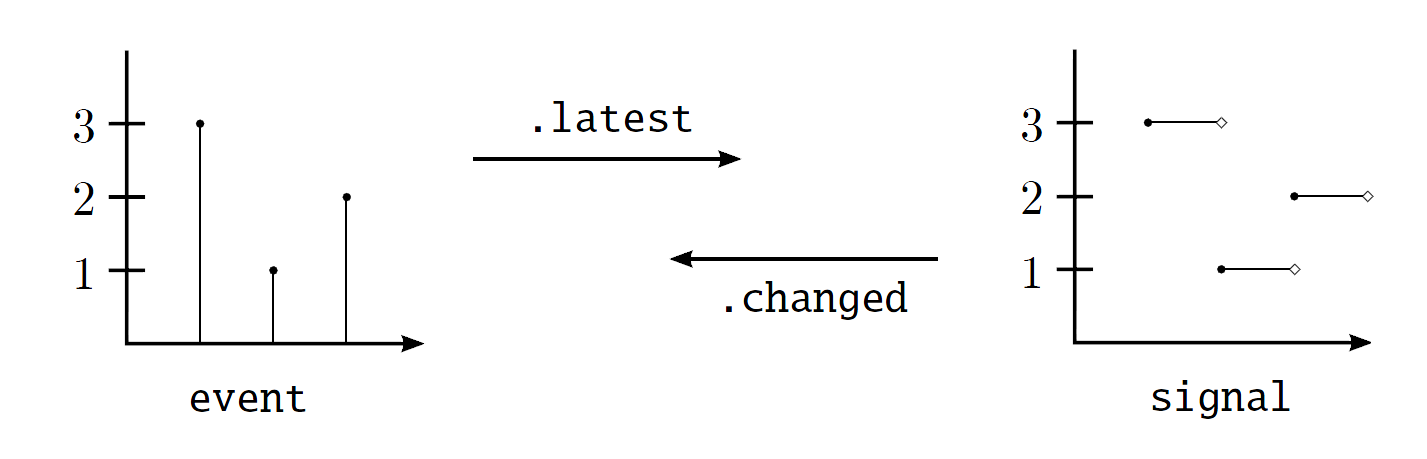
\includegraphics[width=0.98\textwidth]{images/event-signal.png}
\end{center}
\vspace{-6mm}
\caption{Basic conversion functions.}
\label{fig:event-signal}
\end{figure}



\subsubsection{Event to Signal: Latest}
Returns a signal holding the latest value of the event \code{e}. The
initial value of the signal is set to \code{init}.
\\

\code{latest[T](e: Event[T], init: T): Signal[T]}
\\

\noindent
Example:

\begin{codenv}
val e = new ImperativeEvent[Int]()
val s: Signal[Int] = e.latest(10)
assert(s.get == 10)
e(1)
assert(s.get == 1)
e(2)
assert(s.get == 2)
e(1)
assert(s.get == 1)
\end{codenv}


\subsubsection{Signal to Event: Changed}

The \code{changed} function applies to a signal and returns an event
that is fired every time the signal changes its value.
\\

\code{changed[U >: T]: Event[U]}
\\

\noindent
Example:

\begin{codenv}
var test = 0
val v =  Var(1)
val s = Signal{ v() + 1 }
val e: Event[Int] = s.changed
e += ((x:Int)=>{test+=1})
v.set(2)
assert(test == 1)
v.set(3)
assert(test == 2)
\end{codenv}



\subsection{Advanced Conversion Functions}

Some of the conversion functions can be called on a signal providing
an event as the first parameter or can be called on an event providing
a signal as the first parameter. While the behavior is the same, the
signature of the function is obviously different. For example, the
function \code{snapshot} can return a signal that is updated on an
event occurrence. Hence, the function can be exposed both on the
\code{Signal} and the \code{Event} interface. For example:

\begin{codenv}
val e: Event[V]  = ... // An event
val s: Signal[V] = ... // A signal

e.snapshot[V](s: Signal[V]): Signal[V]
s.snapshot[V](e : Event[_]): Signal[V]
\end{codenv}


For simplicity, in those cases, we document the signature of the
function with all the interested objects in the parameters. For
example:

\begin{codenv}
def snapshot[V](e : Event[_], s: Signal[V]): Signal[V]
\end{codenv}


\subsubsection{Fold}
The \code{fold} function creates a signal by folding events with a
given function. Initially the signal holds the \code{init}
value. Every time a new event arrives, the function \code{f} is
applied to the previous previous value of the signal and to the value
associated to the event. The result is the new value of the signal.
\\

\code{fold[T,A](e: Event[T], init: A)(f :(A,T)=>A): Signal[A]}
\\

\noindent
Example:

\begin{codenv}
val e = new ImperativeEvent[Int]()
val f = (x:Int,y:Int)=>(x+y)
val s: Signal[Int] = e.fold(10)(f)
e(1)
e(2)
assert(s.get == 13)
\end{codenv}


\subsubsection{Iterate}
Returns a signal holding the value computed by \code{f} on the
occurrence of an event. Differently from \code{fold}, there is no
accumulator, i.e. the value of the signal does not depend on the
previous values but only on the value carried by the event.
\\

\code{iterate[A](e: Event[\_], init: A)(f: A=>A): Signal[A]}
\\

\noindent
Example:

\begin{codenv}
var test: Int = 0
val e = new ImperativeEvent[Int]()
val f = (x:Int)=>{test=x; x+1}
val s: Signal[Int] = e.iterate(10)(f)
e(1)
assert(test == 10)
assert(s.get == 10)
e(2)
assert(test == 11)
assert(s.get == 10)
e(1)
assert(test == 12)
assert(s.get == 10)
\end{codenv}



\subsubsection{LatestOption}

The \code{latestOption} function is a variant of the \code{latest}
function which uses the \code{Option} type to distinguish the case in
which the event did not fire yet. Holds the latest value of an event
as \code{Some(val)} or \code{None}.
\\

\code{latestOption[T](e: Event[T]): Signal[Option[T]]}
\\

\noindent
Example:

\begin{codenv}
val e = new ImperativeEvent[Int]()
val s: Signal[Option[Int]] = e.latestOption(e)
assert(s.get == None)
e(1)
assert(s.get == Option(1))
e(2)
assert(s.get == Option(2))
e(1)
assert(s.get == Option(1))
\end{codenv}


\subsubsection{Last}

The \code{last} function generalizes the \code{latest} function and
returns a signal which holds the last \code{n} events.
\\

\code{last[T](e: Event[T], n: Int): Signal[List[T]]}
\\

Initially, an empty list is returned. Then the values are
progressively filled up to the size specified by the
programmer. Example:

\begin{codenv}
val e = new ImperativeEvent[Int]()
val s: Signal[List[Int]] = e.last(5)

assert(s.get == List())
e(1)
assert(s.get == List(1))
e(2)
assert(s.get == List(2,1))

e(3);e(4);e(5)
assert(s.get == List(5,4,3,2,1))
e(6)
assert(s.get == List(6,5,4,3,2))
\end{codenv}



\subsubsection{List}
Collects the event values in a (growing) list. This function should be
used carefully. Since the entire history of events is maintained, the
function can potentially introduce a memory overflow.
\\

\code{list[T](e: Event[T]): Signal[List[T]]}




\subsubsection{Count}

Returns a signal that counts the occurrences of the event. Initially,
when the event has never been fired yet, the signal holds the value
0. The argument of the event is simply discarded.
\\

\code{count(e: Event[\_]): Signal[Int]}
\\

\begin{codenv}
val e = new ImperativeEvent[Int]()
val s: Signal[Int] = e.count
assert(s.get == 0)
e(1)
e(3)
assert(s.get == 2)
\end{codenv}




\subsubsection{Snapshot}
Returns a signal updated only when \code{e} fires. If \code{s} in the
meanwhile changes its value, the change is ignored. When the event
\code{e} fires, the resulting signal is updated to the current value
of \code{s}.
\\

\code{snapshot[V](e : Event[\_], s: Signal[V]): Signal[V]}
\\

\noindent
Example:

\begin{codenv}
val e = new ImperativeEvent[Int]()
val v =  Var(1)
val s1 = Signal{ v() + 1 }
val s = e.snapshot(s1)
e(1)
assert(s.get == 2)
v.set(2)
assert(s.get == 2)
e(1)
assert(s.get == 3)
\end{codenv}



\subsubsection{Change}

The \code{change} function is similar to \code{changed}, but it
provides both the old and the new value of the signal in a tuple.
\\

\code{change[U >: T]: Event[(U, U)]}
\\

\noindent
Example:

\begin{codenv}
val s = Signal{ ... }
val e: Event[(Int,Int)] = s.change
e += ((x:(Int,Int))=>{ ... })
\end{codenv}


\subsubsection{ChangedTo}

The \code{changedTo} function is similar to \code{changed}, but it
fires an event only when the signal changes its value to a given
value.
\\

\code{changedTo[V](value: V): Event[Unit]}
\\

\begin{codenv}
var test = 0
val v =  Var(1)
val s = Signal{ v() + 1 }
val e: Event[Unit] = s.changedTo(3)
e += ((x:Unit)=>{test+=1})

assert(test == 0)
v set(2)
assert(test == 1)
v set(3)
assert(test == 1)
\end{codenv}



\subsubsection{Reset}

When the \code{reset} function is called for the first time, the
\code{init} value is used by the factory to determine the signal
returned by the \code{reset} function. When the event occurs the
 factory is applied to the event value to determine the new signal.
\\

\code{reset[T,A](e: Event[T], init: T)(factory: (T)=>Signal[A]):
Signal[A]}
\\

\noindent
Example:

\begin{codenv}
val e = new ImperativeEvent[Int]()
val v1 =  Var(0)
val v2 =  Var(10)
val s1 = Signal{ v1() + 1 }
val s2 = Signal{ v2() + 1 }

def factory(x: Int) = x%2 match {
  case 0 => s1
  case 1 => s2
}
val s3 = e.reset(100)(factory)

assert(s3.get == 1)
v1.set(1)
assert(s3.get == 2)
e(101)
assert(s3.get == 11)
v2.set(11)
assert(s3.get == 12)
\end{codenv}





\subsubsection{Switch/toggle}


The \code{toggle} function switches alternatively between the given
signals on the occurrence of an event \code{e}. The value attached to
the event is simply discarded.
\\

\code{toggle[T](e : Event[\_], a: Signal[T], b: Signal[T]): Signal[T]}
\\


The \code {switchTo} function switches the value of the signal on the
occurrence of the event \code{e}. The resulting signal is a constant
signal whose value is the value carried by the event \code{e}.
\\

\code{switchTo[T](e : Event[T], original: Signal[T]): Signal[T]}
\\

\noindent
The \code{switchOnce} function switches to a new signal provided as a
parameter, once, on the occurrence of the event \code{e}.
\\

\code{switchOnce[T](e: Event[\_], original: Signal[T], newSignal:
  Signal[T]): Signal[T]}
\\





% Not (yet) documented.
% changedTo




\newpage


\section{Common Pitfalls}~\label{sec:pitfalls} In this section we
collect the most common pitfalls for users that are new to reactive
programming and \REScala.


\subsection{Accessing values in signal expressions} The \code{()}
operator used on a signal or a var, inside a signal expression,
returns the signal/var value {\it and} creates a dependency. The
\code{get} operator returns the current value but does {\it not}
create a dependency. For example the following signal declaration
creates a dependency between \code{a} and \code{s}, and a dependency
between \code{b} and \code{s}.
\begin{codenv}
val s = Signal{ a() + b() }
\end{codenv}
The following code instead establishes only a dependency between
\code{b} and \code{s}.
\begin{codenv}
val s = Signal{ a.get + b() }
\end{codenv}
In other words, in the last example, if \code{a} is updated, \code{s}
is not automatically updated. With the exception of the rare cases in
which this behavior is desirable, using \code{get} inside a signal
expression is almost certainly a mistake. As a rule of dumb, signals
and vars appear in signal expressions with the \code{()} operator.


\subsection{Attempting to assign a signal} Signals are not
assignable. Signal depends on other signals and vars, the dependency
is expressed by the signal expression. The value of the signal is
automatically updated when one of the values it depends on
changes. Any attempt to set the value of a signal manually is a
mistake.


\subsection{Side effects in signal expressions} Signal expressions
should be pure. i.e. they should not modify external variables. For
example the following code is conceptually wrong because the variable
\code{c} is imperatively assigned form inside the signal expression
(Line~\ref{assign}).
\begin{codenv}
var c = 0                 /* WRONG - DON'T DO IT */
val s = Signal{
  val sum = a() + b();
  c = sum * 2  (*@\label{assign}@*)
}
 ...
foo(c)
\end{codenv}

A possible solution is to refactor the code above to a more functional
style. For example, by removing the variable \code{c} and replacing it
directly with the signal.
\begin{codenv}
val c = Signal{
  val sum = a() + b();
  sum * 2
}
 ...
foo(c.get)
\end{codenv}



\subsection{Cyclic dependencies} When a signal \code{s} is defined, a
dependency is establishes with each of the signals or vars that appear
in the signal expression of \code{s}. Cyclic dependencies produce a
runtime error and must be avoided. For example the following code:

\begin{codenv}
val a = Var(0)             /* WRONG - DON'T DO IT */
val s = Signal{ a() + t() }
val t = Signal{ a() + s() + 1 }
\end{codenv}

creates a mutual dependency between \code{s} and
\code{t}. Similarly, indirect cyclic dependencies must be avoided.



\subsection{Objects and mutability} Vars and signals may behave
unexpectedly with mutable objects. Consider the following example.

\begin{codenv}
class Foo(init: Int){            /* WRONG - DON'T DO IT */
  var x = init
}
val foo = new Foo(1)

val varFoo = Var(foo)
val s = Signal{ varFoo().x + 10 }
// s.get == 11
foo.x = 2 (*@\label{same}@*)
// s.get == 11
\end{codenv}

One may expect that after increasing the value of \code{foo.x} in
Line~\ref{same}, the signal expression is evaluated again and updated
to 12. The reason why the application behaves differently is that
signals and vars hold {\it references} to objects, not the objects
themselves. When the statement in Line~\ref{same} is executed, the
value of the \code{x} field changes, but the reference hold by the
\code{varFoo} var is the same. For this reason, no change is detected
by the var, the var does not propagate the change to the signal, and
the signal is not reevaluated.

A solution to this problem is to use immutable objects. Since the
objects cannot be modified, the only way to change a filed is to
create an entirely new object and assign it to the var. As a result,
the var is reevaluated.

\begin{codenv}
class Foo(x: Int){}
val foo = new Foo(1)

val varFoo = Var(foo)
val s = Signal{ varFoo().x + 10 }
// s.get == 11
varFoo()= newFoo(2)
// s.get == 12
\end{codenv}

Alternatively, one can still use mutable objects but assign again the
var to force the reevaluation. However this style of programming is
confusing for the reader and should be avoided when possible.

\begin{codenv}
class Foo(init: Int){   /* WRONG - DON'T DO IT */
  var x = init
}
val foo = new Foo(1)

val varFoo = Var(foo)
val s = Signal{ varFoo().x + 10 }
// s.get == 11
foo.x = 2 (*@\label{same}@*)
varFoo()=foo
// s.get == 11
\end{codenv}


\subsection{Functions of reactive values} Functions that operate on
traditional values are not automatically transformed to operate on
signals. For example consider the following functions:

\begin{codenv}
def increment(x: Int): (Int=>Int) = x + 1
\end{codenv}

The following code does not compile because the compiler expects an
integer, not a var as a parameter of the \code{increment} function. In
addition, since the \code{increment} function returns an integer,
\code{b} has type \code{Int}, and the call \code{b()} in the signal
expression is also rejected by the compiler.

\begin{codenv}
val a = Var(1)           /* WRONG - DON'T DO IT */
val b = increment(a)
val s = Signal{ b() + 1 }
\end{codenv}

The following code snippet is syntactically correct, but the signal
has a constant value 2 and is not updated when the var changes.

\begin{codenv}
val a = Var(1)
val b = increment(a.get)
val s = Signal{ b + 1 }
\end{codenv}

The following solution is syntactically correct and the signal
\code{s} is updated every time the var \code{a} is updated.

\begin{codenv}
val a = Var(1)
val s = Signal{ increment(a()) + 1 }
\end{codenv}





\newpage




\section{Technicalities}~\label{sec:technicalities}

This section is meant to cover the implementation details of \REScala
that are necessary to correctly run the current the library.


\subsection{Imports and dependencies}

To work with \REScala programmers need to properly import the reactive
abstractions offered by the language. The following imports are
normally sufficient for all the basic functionalities of \REScala:

\begin{codenv}
import react._
import react.events._
import macro.SignalMacro.{SignalM => Signal}
\end{codenv}

Note that signal expressions are currently implemented as macros,
i.e. the body of a signal expression is analyzed to detect the
reactive values and establish the dependencies. To use macros for
signal expressions, the macro \code{SignalM} is imported and renamed
to \code{Signal} (Line 3).




\newpage



\section{Essential Related Work}~\label{sec:related}


A more academic presentation of \REScala is in \cite{rescala}. A
complete bibliography on reactive programming is beyond the scope of
this work. The interested reader can refer
to~\cite{rective-progr-survey} for an overview of reactive programming
and to~\cite{Salvaneschi:2013:RBO:2451436.2451442} for the issues
concerning the integration of RP with object-oriented programming.


\REScala builds on ideas originally developed in
EScala~\cite{Gasiunas:2011:EME:1960275.1960303} -- which supports
event combination and implicit events. Other reactive languages
directly represent time-changing values and remove inversion of
control. Among the others, we mention
FrTime~\cite{DBLP:conf/esop/CooperK06} (Scheme),
FlapJax~\cite{Meyerovich:2009:FPL:1640089.1640091} (Javascript),
AmbientTalk/R~\cite{ambienttalkR} and
Scala.React~\cite{EPFL-REPORT-148043} (Scala).




\newpage



\section{Acknowledgments}\label{sec:ack}

Several people contributed to this manual with their ideas and
comments. Among the others Gerold Hintz and Pascal Weisenburger.




\newpage



\bibliographystyle{abbrv}
\bibliography{manual}




\end{document}
